\documentclass[11pt]{article}
\usepackage[letterpaper,margin=0.8in]{geometry}
\usepackage{enumitem,array,booktabs,xcolor,tikz,amssymb,amsmath}
\usetikzlibrary{calc,patterns,decorations.pathmorphing,arrows.meta}
\usepackage{needspace}
\usepackage[T1]{fontenc}\usepackage{lmodern}
\setlength{\parindent}{0pt}\setlength{\parskip}{5pt}
\renewcommand{\arraystretch}{1.5}
\newif\ifkey \input{mode}
\newcommand{\ans}[2][1]{\ifkey{\color{red!70!black}\itshape #2}\par\else\par\foreach\i in{1,...,#1}{\vspace{0.75cm}\noindent\rule{\linewidth}{0.4pt}\par}\fi}
\newcommand{\work}[2][3cm]{\ifkey{\color{red!70!black}\itshape #2}\par\else\par\vspace{#1}\fi}
\newcommand{\fa}[1]{\ifkey{\color{red!70!black}\bfseries #1}\else\fi}
\newcommand{\blank}[2][2.5cm]{\ifkey\fa{#2}\else\rule{#1}{0.4pt}\fi}
\newcommand{\pts}[1]{\hfill{\small[#1]}}
\newcommand{\sect}[1]{\par\needspace{22\baselineskip}\vspace{8pt}\noindent{\large\bfseries #1}\par\vspace{-4pt}\noindent\rule{\linewidth}{0.8pt}\par}
\newcommand{\q}[1]{\par\needspace{8\baselineskip}\vspace{6pt}\noindent\textbf{#1}\ }
\newcommand{\sub}[1]{\par\vspace{3pt}\hspace*{1em}(#1)\ }
\tikzset{grnd/.style={pattern=north east lines,draw=none},
  frc/.style={-{Stealth[length=7pt]},very thick,red!70!black}}

\pagestyle{plain}
\begin{document}
\ifkey{\color{red!70!black}\bfseries ANSWER KEY}\par\fi
{\LARGE\bfseries Forces Test: Friction, Inclines, Systems and Springs}\par\vspace{6pt}
Name: \rule{6.5cm}{0.4pt}\hfill Date: \rule{3cm}{0.4pt}\par
Calculators allowed. Show your work and units. Use $g = 9.8\ \text{m/s}^2$. Total: 39 points.

\begin{center}\fbox{\parbox{0.9\linewidth}{\centering
$\Sigma F = ma \qquad W = mg \qquad f_k = \mu_k N \qquad f_s \le \mu_s N \qquad F = kx$}}\end{center}

\sect{Part A: Third law and tension}
\q{1.} A tow truck pulls a car forward with a force of 800 N.
\sub{a} How big is the force the car exerts on the truck, and which way does it point? \pts{1}\par
\blank[7cm]{800 N, backward (toward the car).}
\sub{b} If the two forces are equal and opposite, why can the car still speed up? \pts{1}
\ans{They act on different objects, so they do not cancel. Only the forces on the car decide its motion: the 800 N pull is bigger than the friction on the car.}

\q{2.} A 5.0 kg bag hangs at rest from an ideal rope that runs over an ideal pulley to a hook on the wall. What is the tension in the rope at the hook? \pts{1}\par
\blank[4cm]{49 N (same tension all along an ideal rope: $T = mg = 5.0 \times 9.8$).}

\sect{Part B: Friction}
\q{3.} A 20 kg box sits on a floor. $\mu_s = 0.50$ and $\mu_k = 0.30$.\par
\begin{center}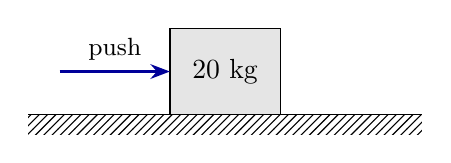
\begin{tikzpicture}
\fill[grnd] (0,-0.25) rectangle (5,0); \draw (0,0)--(5,0);
\draw[fill=gray!20] (1.8,0) rectangle (3.2,1.1) node[midway]{20 kg};
\draw[frc,blue!60!black] (0.4,0.55)--(1.8,0.55) node[midway,above,black]{\small push};
\end{tikzpicture}\end{center}
\sub{a} Find the normal force on the box. \pts{1} \hfill \blank{196 N}
\sub{b} What is the largest static friction the floor can give? \pts{1} \hfill \blank{98 N ($0.50 \times 196$)}
\sub{c} You push with 60 N and the box does not move. How big is the friction force? Explain. \pts{2}
\ans{60 N. Static friction only matches the push, up to its 98 N limit; the box is at rest, so the net force is zero.}
\sub{d} Now you push with 120 N. First say in words whether the box moves and why. Then find its acceleration. \pts{4}
\work[3.2cm]{Moves: 120 N is more than the 98 N static limit (1). Once sliding, $f_k = 0.30 \times 196 = 58.8$ N (1). $a = (120 - 58.8)/20$ (1) $= 3.1\ \text{m/s}^2$ (1).}

\q{4.} Draw the friction force on each object as an arrow. \pts{2}\par
\begin{center}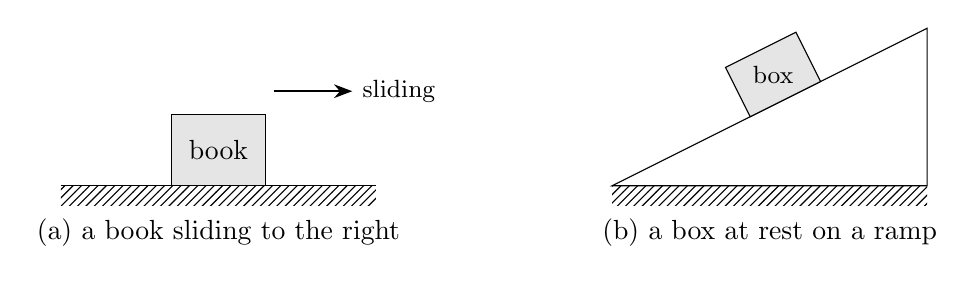
\begin{tikzpicture}
\begin{scope}
\fill[grnd] (0,-0.25) rectangle (4,0); \draw (0,0)--(4,0);
\draw[fill=gray!20] (1.4,0) rectangle (2.6,0.9) node[midway]{book};
\draw[-{Stealth},thick] (2.7,1.2)--(3.7,1.2) node[right]{\small sliding};
\ifkey\draw[frc] (1.4,0.15)--(0.5,0.15);\fi
\node at (2,-0.6) {(a) a book sliding to the right};
\end{scope}
\begin{scope}[xshift=7cm]
\fill[grnd] (0,0)--(4,0)--(4,-0.25)--(0,-0.25)--cycle;
\draw (0,0)--(4,0)--(4,2)--cycle;
\begin{scope}[shift={(2.2,1.1)},rotate=26.57]\draw[fill=gray!20] (-0.5,0) rectangle (0.5,0.7) node[midway]{\small box};
\ifkey\draw[frc] (0.5,0.1)--(1.4,0.1);\fi\end{scope}
\node at (2,-0.6) {(b) a box at rest on a ramp};
\end{scope}
\end{tikzpicture}\end{center}
\ifkey{\color{red!70!black}\itshape (a) to the left, against the sliding. (b) up the ramp, against the way it would slide.}\par\fi

\sect{Part C: Inclines}
\q{5.} A 10 kg crate sits on a frictionless ramp tilted at $30^\circ$.\par
\begin{center}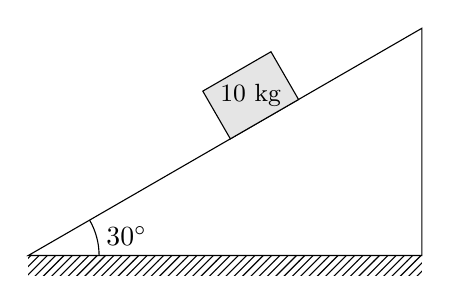
\begin{tikzpicture}
\fill[grnd] (0,-0.25) rectangle (5,0);
\draw (0,0)--(5,0)--(5,2.887)--cycle;
\draw (0.9,0) arc (0:30:0.9); \node at (1.25,0.25) {$30^\circ$};
\begin{scope}[shift={(3,1.732)},rotate=30]\draw[fill=gray!20] (-0.5,0) rectangle (0.5,0.7) node[midway]{\small 10 kg};\end{scope}
\end{tikzpicture}\end{center}
\sub{a} Draw the free-body diagram of the crate. Name the object that exerts each force. \pts{2}
\work[2.6cm]{Weight (Earth), straight down; normal force (ramp), perpendicular to the ramp surface. No friction.}
\sub{b} Find the part of the weight that points down the ramp. \pts{1} \hfill \blank{49 N ($mg\sin 30^\circ$)}
\sub{c} Find the normal force. \pts{1} \hfill \blank{85 N ($mg\cos 30^\circ$)}
\sub{d} Find the crate's acceleration. \pts{1} \hfill \blank{$4.9\ \text{m/s}^2$ down the ramp}
\sub{e} The ramp is raised to $40^\circ$. Does the normal force go up or down? Why? \pts{1}
\ans{Down: less of the weight presses into a steeper ramp ($\cos\theta$ gets smaller), so the ramp pushes back less.}

\sect{Part D: Connected objects}
\q{6.} A 3.0 kg cart on a frictionless table is tied to a 1.0 kg mass that hangs over an ideal pulley.\par
\begin{center}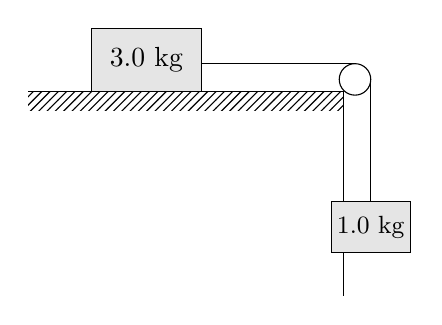
\begin{tikzpicture}
\fill[grnd] (0,-0.25) rectangle (4,0); \draw (0,0)--(4,0)--(4,-2.6);
\draw[fill=gray!20] (0.8,0) rectangle (2.2,0.8) node[midway]{3.0 kg};
\draw (4.15,0.15) circle (0.2); \draw (2.2,0.35)--(4.15,0.35); \draw (4.35,0.15)--(4.35,-1.4);
\draw[fill=gray!20] (3.85,-1.4) rectangle (4.85,-2.05) node[midway]{\small 1.0 kg};
\end{tikzpicture}\end{center}
\sub{a} Before calculating: will the acceleration be more than $g$, less than $g$, or equal to $g$? Why? \pts{1}
\ans{Less than $g$: the hanging weight has to speed up both masses, not just itself.}
\sub{b} Treat the two masses as one system. Find the acceleration. \pts{2}
\work[2.4cm]{$a = \dfrac{m_2 g}{m_1 + m_2} = \dfrac{1.0 \times 9.8}{4.0} = 2.45\ \text{m/s}^2$ (2.5 is fine).}
\sub{c} Now look at the cart alone. Find the tension in the string. \pts{2}
\work[2.4cm]{$T = m_1 a = 3.0 \times 2.45 = 7.4$ N.}
\sub{d} Is the tension more or less than the weight of the hanging mass? Why does that make sense? \pts{1}
\ans{Less (7.4 N vs 9.8 N). The hanging mass speeds up downward, so the net force on it is down: its weight must beat the tension.}

\q{7.} An Atwood machine: a 5.0 kg mass and a 3.0 kg mass hang on either side of an ideal pulley. Find the acceleration and the tension. \pts{4}
\work[3.4cm]{$a = \dfrac{(5.0 - 3.0)(9.8)}{8.0} = 2.45\ \text{m/s}^2$ (2). For the 3.0 kg mass: $T - 29.4 = 3.0 \times 2.45$, so $T = 36.8$ N (2). Check with the 5.0 kg mass: $49 - T = 5.0 \times 2.45$, $T = 36.8$ N.}

\sect{Part E: Springs}
\q{8.} A student hangs weights on a spring and measures the stretch.\par
\begin{center}\begin{tabular}{|l|*{4}{>{\centering\arraybackslash}p{1.4cm}|}}\hline
Force (N) & 0 & 2.0 & 4.0 & 6.0\\\hline
Stretch (m) & 0 & 0.040 & 0.080 & 0.120\\\hline
\end{tabular}\end{center}
\sub{a} Find the spring constant $k$. \pts{2} \hfill \blank{50 N/m (slope: $2.0/0.040$)}
\sub{b} Predict the stretch when a 1.5 kg mass hangs at rest on this spring. \pts{2}
\work[2.4cm]{$F = mg = 14.7$ N; $x = F/k = 14.7/50 = 0.29$ m.}

\q{9.} Spring P has $k = 200$ N/m and spring Q has $k = 400$ N/m. Each is pulled with 10 N. Which stretches more, and by how much more? \pts{2}
\work[2.2cm]{P: $10/200 = 0.050$ m. Q: $10/400 = 0.025$ m. P stretches 0.025 m more (twice as far).}

\sect{Stretch}
\q{10.} Ski patrol lowers a rescue sled down a snowy $25^\circ$ slope with a rope that runs parallel to the slope. The sled and patient together have a mass of 90 kg, $\mu_k = 0.10$, and the sled moves down at a constant speed.\par
\sub{a} Before calculating: is the rope tension more or less than the part of the weight along the slope? Why? \pts{1}
\ans{Less. Friction also points up the slope and helps hold the sled back.}
\sub{b} Find the tension in the rope. \pts{3}
\work[4cm]{Constant speed, so $\Sigma F = 0$ along the slope. $mg\sin 25^\circ = 373$ N down the slope (1). $f_k = 0.10 \times mg\cos 25^\circ = 80$ N up the slope (1). $T = 373 - 80 = 293$ N (1).}
\end{document}
